\section{Convolution}

The implementation of this function has the following signature:

\begin{lstlisting}[language=python][h!]
convolve(img_input, kernel, padding_type = 'zero', padding_color = 0, normalize = False):
\end{lstlisting}

The kernels tested are shown in figure \ref{fig:conv-kernels}.
 
\begin{figure}[h!]
\centering
\begin{subfigure}{0.3\textwidth}
  \centering
  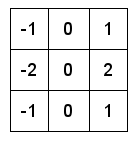
\includegraphics[width=0.5\linewidth]{figs/sobel.png}
  \caption{Sobel 3x3}
\end{subfigure}%
\begin{subfigure}{0.3\textwidth}
  \centering
  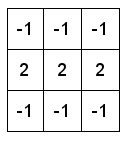
\includegraphics[width=0.5\linewidth]{figs/line.png}
  \caption{Line detector 3x3}
\end{subfigure}%
\begin{subfigure}{0.3\textwidth}
  \centering
  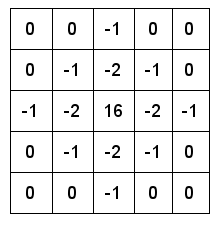
\includegraphics[width=0.5\linewidth]{figs/laplacian-of-gaussian.png}
  \caption{Laplacian of Gaussian 5x5}
\end{subfigure}
\begin{subfigure}{0.3\textwidth}
  \centering
  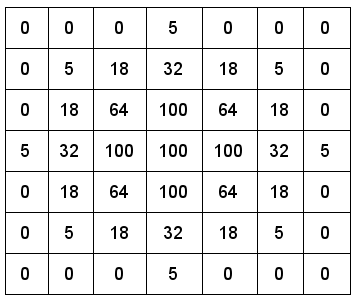
\includegraphics[width=0.9\linewidth]{figs/gaussian.png}
  \caption{Gaussian 7x7}
\end{subfigure}%
\begin{subfigure}{0.7\textwidth}
  \centering
  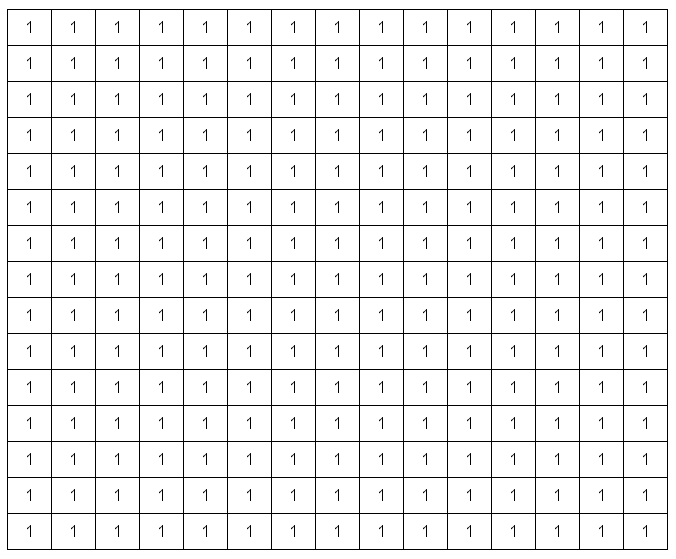
\includegraphics[width=0.9\linewidth]{figs/media.png}
  \caption{Media 15x15}
\end{subfigure}
 \caption{Kernels used in experiments}
\label{fig:conv-kernels}
\end{figure}

Results for each kernel are shown in figure \ref{fig:conv-results}. In the case of the sobel kernel, it corresponds to the vertical component (sobel filter has vertical and horizontal components), thus the results highlights the vertical lines (more clear in the wall of brick). Analyzing the pattern in the line detector it seems like an horizontal line, thus in the result of this kernel, vertical lines disappears. In the case of the Laplacian of Gaussian (LoG) it is working as an edge detector. In the media and Gaussian the results are blurred images, but in the case of the media kernel the result is bigger because of the size of the kernel.

\begin{figure}[h!]
\centering
\begin{subfigure}{0.3\textwidth}
  \centering
  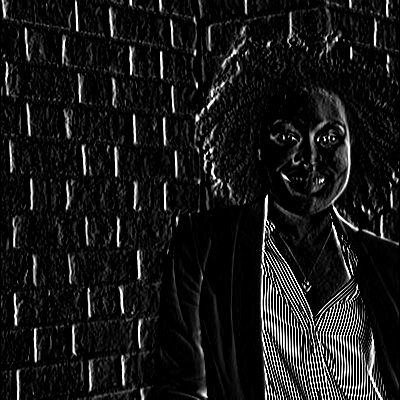
\includegraphics[width=0.9\linewidth]{output/sobel.jpg}
  \caption{Sobel}
\end{subfigure}%
\begin{subfigure}{0.3\textwidth}
  \centering
  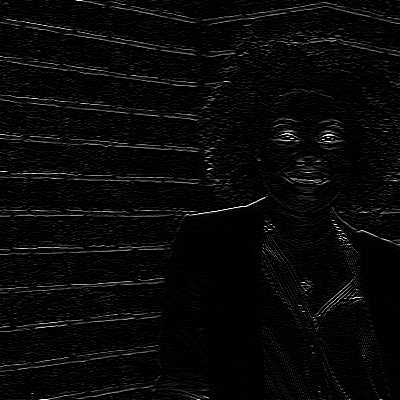
\includegraphics[width=0.9\linewidth]{output/horizontalLine.jpg}
  \caption{Line detector}
\end{subfigure}%
\begin{subfigure}{0.3\textwidth}
  \centering
  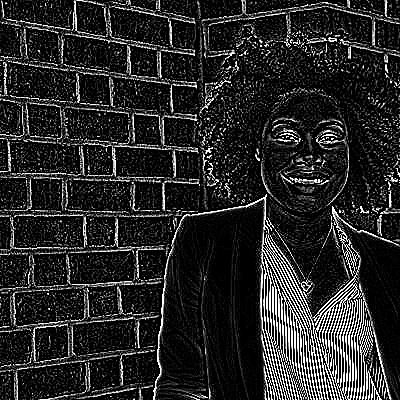
\includegraphics[width=0.9\linewidth]{output/laplasOfGaussi.jpg}
  \caption{Laplacian of Gaussian}
\end{subfigure}
\begin{subfigure}{0.5\textwidth}
  \centering
  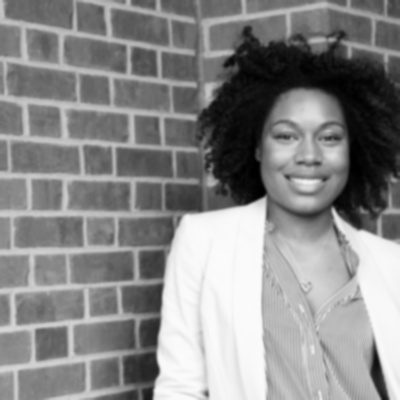
\includegraphics[width=0.5\linewidth]{output/gaussian.jpg}
  \caption{Gaussian}
\end{subfigure}%
\begin{subfigure}{0.5\textwidth}
  \centering
  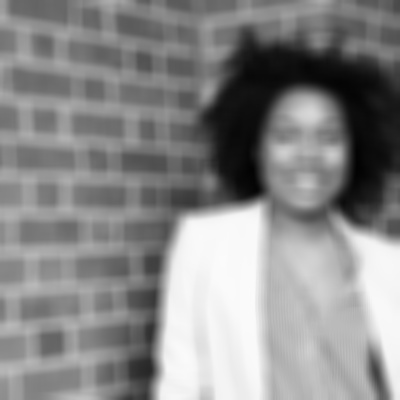
\includegraphics[width=0.5\linewidth]{output/media.jpg}
  \caption{Media} 
\end{subfigure}
 \caption{Results of convolution}
\label{fig:conv-results}
\end{figure}

Different kinds of padding are available: $zero, mirror$ and $constant$, the results for different padding strategies are shown in figure \ref{fig:padding-strategy}.

The zero padding suffers of white borders, this may not be logical since 0 is equivalent to black, but if we analyze the convolution kernel (laplacian of gaussian) it makes sense. Mirror padding has the best results because it does not saturate the borders with an specific color. Contrary to zero padding, the constant padding with $c=255$ turns the borders black, the constant padding with $c=128$ has the most similar result to mirror approach.

Because of these results, we consider mirror padding in future experiments.

\begin{figure}[h!]
\centering
\begin{subfigure}{0.25\textwidth}
  \centering
  \frame{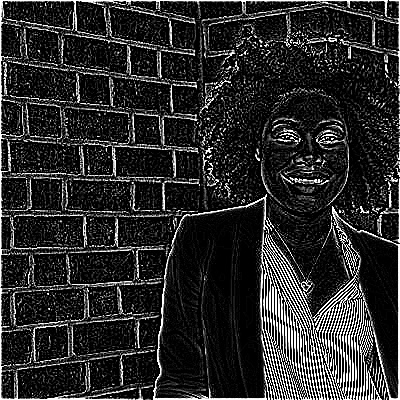
\includegraphics[width=0.9\linewidth]{output/zero.jpg}}
  \caption{Zero padding}
\end{subfigure}%
\begin{subfigure}{0.25\textwidth}
  \centering
  \frame{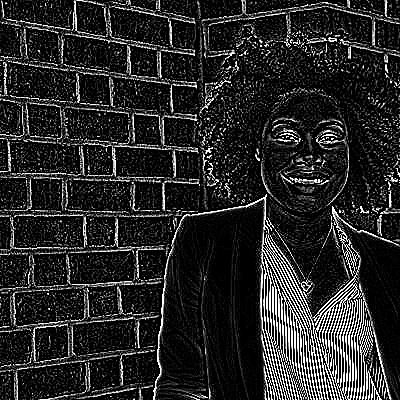
\includegraphics[width=0.9\linewidth]{output/mirror.jpg}}
  \caption{Mirror padding}
\end{subfigure}%
\begin{subfigure}{0.25\textwidth}
  \centering
  \frame{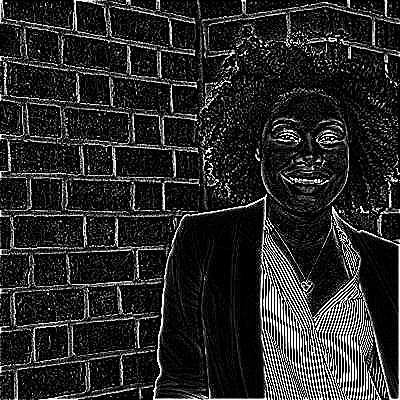
\includegraphics[width=0.9\linewidth]{output/constant128.jpg}}
  \caption{Constant padding $C = 128$}
\end{subfigure}%
\begin{subfigure}{0.25\textwidth}
  \centering
  \frame{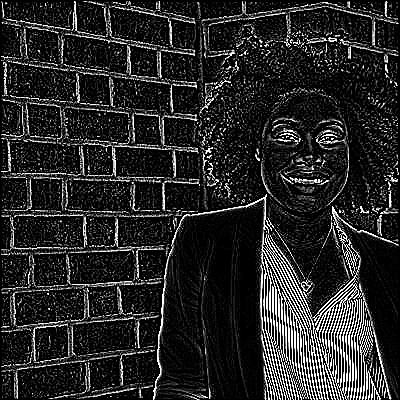
\includegraphics[width=0.9\linewidth]{output/constant255.jpg}}
  \caption{Constant padding $C = 255$}
\end{subfigure}
 \caption{Padding results with Laplacian of Gaussian filter}
\label{fig:padding-strategy}
\end{figure}

\vspace{2cm}

The measure of the execution time of the convolution function is shown in table~\ref{tab:time_execution}. Note that since two images are $300 \times 300$ and the other two are $400 \times 400$, we evaluate the time using one of each dimension. In the same way, we consider only one kernel of $ 3 \times 3$ out of the original three.

From the table we can see that the our implementation is much more slower than the OpenCV one, this is because the OpenCV library has its methods optimized, an option to improve our implementation is to use $cython$\footnote{\url{http://www.pyimagesearch.com/2017/08/28/fast-optimized-for-pixel-loops-with-opencv-and-python/} shows a solution for this problem.}

\begin{table}[h!]
\centering
\begin{tabular}{|l|l|l|c|r|r|r|}
\hline
\multicolumn{2}{|c|}{\textit{\textbf{Image}}} & \multicolumn{2}{c|}{\textit{\textbf{kernel}}} & \multicolumn{2}{c|}{\textit{\textbf{execution time(seconds)}}} & \multicolumn{1}{c|}{\multirow{2}{*}{\textit{\textbf{Speedup}}}} \\ \cline{1-6}
\multicolumn{1}{|c|}{\textit{\textbf{name}}} & \multicolumn{1}{c|}{\textit{\textbf{dimension}}} & \multicolumn{1}{c|}{\textit{\textbf{name}}} & \textit{\textbf{dimension}} & \multicolumn{1}{c|}{\textit{\textbf{\begin{tabular}[c]{@{}c@{}}Our \\ implementation\end{tabular}}}} & \multicolumn{1}{c|}{\textit{\textbf{OpenCV}}} & \multicolumn{1}{c|}{} \\ \hline
\multirow{4}{*}{p1-1-1.jpg} & \multirow{4}{*}{400x400} & Sobel & 3x3 & 1.0571 & 0.0002 & 5285.5 \\ \cline{3-7} 
 &  & Laplacian of gaussian & 5x5 & 1.1044 & 0.0004 & 2761 \\ \cline{3-7} 
 &  & Gaussian & 7x7 & 1.1191 & 0.0008 & 1398 \\ \cline{3-7} 
 &  & Media & 15x15 & 1.2273 & 0.0026 & 472 \\ \hline
\multirow{4}{*}{p1-1-2.png} & \multirow{4}{*}{300x300} & Sobel & 3x3 & 0.5934 & 0.0001 & 5934 \\ \cline{3-7} 
 &  & Laplacian of gaussian & 5x5 & 0.6023 & 0.0002 & 3011 \\ \cline{3-7} 
 &  & Gaussian & 7x7 & 0.6175 & 0.0004 & 1543 \\ \cline{3-7} 
 &  & Media & 15x15 & 0.7376 & 0.0024 & 307 \\ \hline
\end{tabular}
\caption{Measures of the execution time}
\label{tab:time_execution}
\end{table}

